\chapter{Криві другого порядку}

Загальне рівняння кривої другого порядку має такий вигляд:

$$Ax^2 + By^2 + Cxy + Dx + Ey + F = 0$$

При різних значеннях коефіцієнтів можемо отримати вироджені випадки:
прямі, точки, криві лінії. Ми ж будемо розглядати невироджені випадки кривих
другого порядку – еліпс, гіперболу, параболу. 

\section{Канонічне рівняння еліпса}

\begin{definition}
	Еліпсом називається геометричне місце точок площини таких, що сума
	відстаней від кожної з яких до двох фіксованих точок (фокусів) є величина стала. 
\end{definition}

\noindent\parbox{4cm}{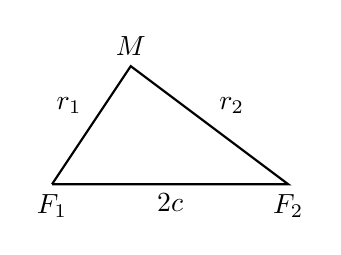
\begin{tikzpicture}[scale=0.5]
	\draw[thick] (-3,0)node[below]{$F_1$} -- (-1,3)node[above]{$M$} -- (3,0)node[below]{$F_2$} -- (-3,0);
	\draw (-2,2)node[left]{$r_1$};
	\draw (1,2)node[right]{$r_2$};
	\draw (0,0)node[below]{$2c$};
\end{tikzpicture}}
\parbox{\textwidth - 4.1cm}{
	Отже, маємо два фокуси $F_1$ і $F_2$, відстань між ними $|F_1F_2| = 2c$. Нехай $M$ – довільна точка
	еліпса. Відрізки $r_1 = |F_1M|$ та $r_2 = |F_2M|$
	називаються фокальними радіусами точки $M$.

	За означенням еліпса: $r_1 + r_2 = 2a$.
}

З трикутника $F_1MF_2$ маємо: $|F_1M| + |F_2M| > |F_1F_2|$, тобто $2a > 2c$, або $a>c$.

\noindent\parbox{6cm}{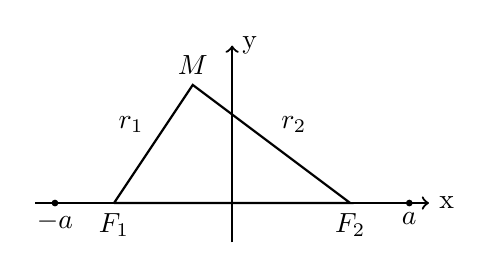
\begin{tikzpicture}[scale=0.5]
	\draw[->, thick] (-5,0) -- (5,0)node[right]{x};
	\draw[->, thick] (0,-1) -- (0,4)node[right]{y};
  	
  	%\draw (-5,-2) grid (5,5);
	\draw[thick] (-3,0)node[below]{$F_1$} -- (-1,3)node[above]{$M$} -- (3,0)node[below]{$F_2$} -- (-3,0);
	\draw (-2,2)node[left]{$r_1$};
	\draw (1,2)node[right]{$r_2$};
	
	\filldraw[black] (-4.5,0) circle(2pt) node[below]{$-a$};
	\filldraw[black] (4.5,0) circle(2pt) node[below]{$a$};
\end{tikzpicture}}
\parbox{\textwidth - 6.1cm}{
	Побудуємо декартову систему
	координат. Нехай вісь $OX$
	пройде через фокуси $F_1$ і $F_2$ ,а
	вісь $OY$ --- через середину
	відрізка $F_1F_2$ . Відповідно до
	вибраної системи координат
	фокуси будуть мати такі
	координати: $F_1(-c,0), F_2(c,0)$. 
}

Оскільки точка $M$ --- це довільна точка еліпса, то вона має координати $(x,y)$. Тоді

$$r_1 = |F_1M| = \sqrt{(x+c)^2+y^2}, r_2 = |F_2M| = \sqrt{(x-c)^2+y^2}.$$

Враховуючи умову $r_1 + r_2 = 2a$, маємо рівняння еліпса:

$$\sqrt{(x+c)^2+y^2} + \sqrt{(x-c)^2+y^2} = 2a.$$

Піднесемо до квадрату обидві частини рівняння:

$$(x+c)^2+y^2 + (x-c)^2+y^2 + 2\sqrt{((x+c)^2+y^2)((x-c)^2+y^2)} = 4a^2.$$

Перегрупувавши доданки, маємо:

$$x^2 + 2xc + c^2 + y^2 + x^2 - 2xc + c^2 + y^2 - 4a^2 = $$

$$= -2\sqrt{((x^2 + y^2 + c^2) + 2xc)((x^2 + y^2 + c^2) - 2xc)}.$$

Виконавши елементарні перетворення, отримаємо: 

$$\sqrt{(x^2 + y^2 + c^2)^2 - 4x^2c^2} = 2a^2 - (x^2 + y^2 + c^2).$$

Знову піднесемо до квадрату та отримаємо:

$$(x^2 + y^2 + c^2)^2 - 4x^2c^2 = (x^2 + y^2 + c^2)^2 + 4a^4 - 4a^2(x^2 + y^2 + c^2).$$

\begin{center}
	або
\end{center}	
	
$$x^2(a^2 - c^2) + y^2a^2 = a^4 - a^2c^2.$$

Позначивши $b^2 = a^2 - c^2$ (оскільки $a>c$), маємо: $x^2b^2 + y^2a^2 = a^2b^2$.
Поділивши обидві частини цієї рівності на $a^2b^2$, отримуємо \textbf{канонічне рівняння
еліпса:}

\begin{wrapfigure}{l}{4.5cm}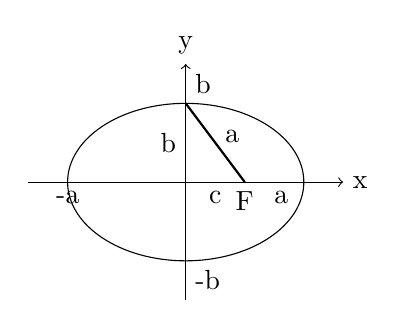
\begin{tikzpicture}[scale=0.5]
	\draw[->] (-4,0) -- (4,0)node[right]{x};
	\draw[->] (0,-3) -- (0,3)node[above]{y};
  	
	\draw (0,0) ellipse (3cm and 2cm);
	\draw[thick] (0,2) -- (1.5,0);
	
	\draw (-3,0)node[below]{-a};
	\draw (0,2)node[above right]{b};
	\draw (1.5,0)node[below]{F};
	\draw (0,-2)node[below right]{-b};
	\draw (2,0)node[below right]{a};
	\draw (0.75,0)node[below]{c};
	\draw (0,1)node[left]{b};
	\draw (0.75,0.75)node[above right]{a};
\end{tikzpicture}\end{wrapfigure}

$$\dfrac{x^2}{a^2} + \dfrac{y^2}{b^2} = 1.$$

Дослідимо форму еліпса. З отриманого рівняння
випливає, що для всіх точок еліпса
$x^2 \leqslant a^2$, $y^2 \leqslant b^2$, або $|x| \leqslant a$, $|y| \leqslant b$, тобто це
означає, що всі точки еліпса знаходяться всередині
прямокутника, сторони якого паралельні осям координат і мають довжини $2a$ та
$2b$, де $a$ --- це \textbf{велика піввісь}, $b$ --- \textbf{мала піввісь} ($a>b$). Кожна точка
$(a,0)$, $(-a,0)$, $(0,b)$, $(0,-b)$, в якій еліпс перетинає осі координат, --- це
\textbf{полюс еліпса (або вершина еліпса)}. Якщо довільні значення $(x,y)$, задовольняють
канонічне рівняння еліпса, то очевидно, що значення $(-x,y)$, $(x,-y)$, $(-x,-y)$ теж будуть
задовольняти рівняння еліпса. Це означає, що координатні осі, кожна з них --- це \textbf{вісь
симетрії}, а точка $O(0,0)$ --- \textbf{центр симетрії еліпса}. 

\section{Канонічне рівняння гіперболи}

\begin{definition}
	\textbf{Гіпербола} --- це геометричне місце точок площини, для яких
	модуль різниці відстаней від двох фіксованих точок (фокусів) є сталою величиною.
\end{definition}

Нехай $F_1$ і $F_2$ --- фокуси, відстань між якими $|F_1F_2| = 2c$, $M$ --- довільна точка
гіперболи, $r_1$ та $r_2$ --- це фокальні радіуси точки $M$.
Згідно з означенням гіперболи $|r_1 - r_2| = 2a$.
З трикутника $F_1MF_2$ маємо: $2a < 2c$, тобто $a < c$.
Побудову декартової системи координат і подальші
викладки здійснюємо так само, як і при виведенні рівняння еліпса:

$$F_1(-c,0), F_2(c,0), M(x,y),$$

$$r_1 = \sqrt{(x + c)^2 + y^2}, r_2 = \sqrt{(x - c)^2 + y^2},$$

$$|r_1 - r_2| = 2a,$$

$$|\sqrt{(x + c)^2 + y^2} - \sqrt{(x - c)^2 + y^2}| - 2a,$$

$$(x^2 + y^2 + c^2) + 2xc + (x^2 + y^2 + c^2) - 2xc -$$

$$-2\sqrt{((x^2+y^2+c^2)+2xc)((x^2+y^2+c^2)-2xc)} =4a^2,$$

$$(x^2+y^2+c^2) - 2a^2 = \sqrt{v^2 - 4x^2c^2},$$

$$(x^2+y^2+c^2) - 4a^2(x^2+y^2+c^2) + 4a^4 = (x^2+y^2+c^2)^2 - 4x^2c^2,$$

$$x^2c^2 - x^2a^2 - y^2a^2 = a^2c^2 - a^4,$$

$$x^2(c^2 - a^2) - y^2a^2 = a^2(c^2 - a^2).$$

Позначимо $B^2 C^2 - A^2$ (враховуючи, що $c>a$). Тоді

$$x^2b^2 - y^2a^2 = a^2b^2.$$

В результаті перетворень отримали \textbf{канонічне рівняння гіперболи}:

$$\dfrac{x^2}{a^2} - \dfrac{y^2}{b^2} = 1$$

З отриманого рівняння випливає, що

$$x^2 = a^2\left(1 + \dfrac{y^2}{b^2}\right) \Rightarrow x \leqslant -a \text{ або } x \geqslant a.$$

Аналогічно,

$$y^2 = b^2\left(\dfrac{x^2}{a^2} - 1\right) \Rightarrow y = \pm\dfrac{b}{a}\sqrt{x^2 - a^2} \Rightarrow y \in (-\infty; +\infty).$$

\begin{wrapfigure}{l}{4.5cm}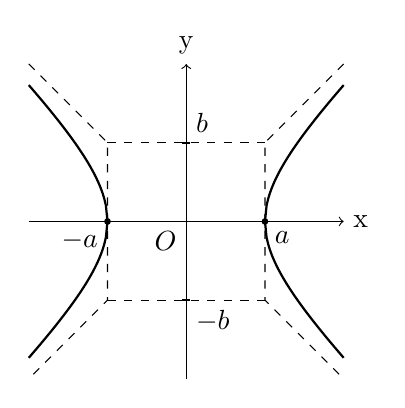
\begin{tikzpicture}[scale=0.5]
	\draw[->] (-4,0) -- (4,0)node[right]{x};
	\draw[->] (0,-4) -- (0,4)node[above]{y};
	
	\def\a{2};
	\def\b{2};
	
	\draw[domain=\a:4, samples=50, thick] plot (\x,{(\b/\a)*sqrt(\x^2 - \a^2)});
	\draw[domain=\a:4, samples=50, thick] plot (\x,{-(\b/\a)*sqrt(\x^2 - \a^2)});
	\draw[domain=\a:4, samples=50, thick] plot ({-\x},{(\b/\a)*sqrt(\x^2 - \a^2)});
	\draw[domain=\a:4, samples=50, thick] plot ({-\x},{-(\b/\a)*sqrt(\x^2 - \a^2)});
	
	\draw[dashed] (-4,4) -- (-2,2) -- (-2,-2) -- (-4,-4);
	\draw[dashed] (4,4) -- (2,2) -- (2,-2) -- (4,-4);
	\draw[dashed] (-2,2) -- (2,2);
	\draw[dashed] (-2,-2) -- (2,-2);
	
	\filldraw[black] (2,0) circle(2pt) node[below right]{$a$};
	\filldraw[black] (-2,0) circle(2pt) node[below left]{$-a$};
	\draw[thick] (-0.1,2) -- (0.1,2);
	\draw[thick] (-0.1,-2) -- (0.1,-2);
	\draw (0,2)node[above right]{$b$};
	\draw (0,-2)node[below right]{$-b$};
	\draw (0,0)node[below left]{$O$};
\end{tikzpicture}\end{wrapfigure}

Тобто гіпербола є необмеженою
кривою, яка складається з двох гілок,
які є симетричними відносно осі $OY$ і
лежать праворуч від прямої $x = a$ та
ліворуч від прямої $x = -a$.

Координатні осі --- це осі симетрії, точка
$O$ --- центр симетрії гіперболи.
Асимптотами гіперболи є прямі
$y = \pm\dfrac{b}{a}x$.

Доведемо це для гілки гіперболи, що лежить у першій чверті: 

$$\dfrac{y^2}{b^2} = \dfrac{x^2}{a^2} - 1 \Rightarrow y = \dfrac{b}{a}\sqrt{x^2 - a^2},$$

тобто

$$\lim\limits_{x \rightarrow +\infty}\dfrac{\dfrac{b}{a}\sqrt{x^2-a^2}}{\dfrac{b}{a}x}
= \lim\limits_{x \rightarrow +\infty}\sqrt{1 - \dfrac{a^2}{x^2}} = 1.$$

Це означає, що чисельник наближається до знаменника, тобто крива при
$x \rightarrow +\infty$ наближається до своєї асимптоти. Для трьох інших чвертей викладки
аналогічні. 

\section{Канонічне рівняння параболи}

\begin{definition}
	\textbf{Парабола} --- це геометричне місце точок площини, кожна з яких
	однаково віддалена від фіксованої точки (фокуса) і від даної прямої (директриси).
\end{definition}

Відстань від фокуса $F$ до директриси $D$ позначимо $p$. Нехай $M$ --- довільна
точка параболи. Тоді $r = |FM|$ --- фокальний радіус точки $M$.

\noindent\parbox{4.5cm}{
	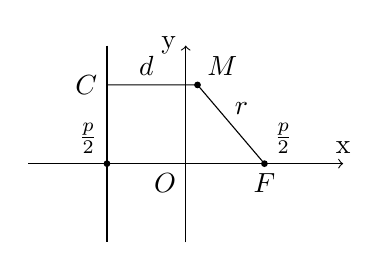
\begin{tikzpicture}[scale=0.5]
		\draw[->] (-4,0) -- (4,0)node[above]{x};
		\draw[->] (0,-2) -- (0,3)node[left]{y};

		\draw (0,0)node[below left]{$O$};
		\draw (-2,3) -- (-2,-2);
		\draw (-2,2)node[left]{$C$} -- (0.3,2)node[above right]{$M$} -- (2,0)node[below]{$F$};
		\filldraw[black] (0.3,2) circle(2pt);	
		\filldraw[black] (-2,0) circle(2pt) node[above left]{$\frac{p}{2}$};
		\filldraw[black] (2,0) circle(2pt) node[above right]{$\frac{p}{2}$};
		\draw (-1,2) node[above]{$d$};
		\draw (1,1) node[above right]{$r$};
	\end{tikzpicture}
}\parbox{\textwidth - 4.5cm}{
	Декартову систему координат будуємо
	таким чином: вісь $OX$ проходить через
	фокус $F$ перпендикулярно директрисі $D$, а
	вісь $OY$ --- через середину відстані від $F$ до
	$D$. Тоді $M(x,y)$, $F(\frac{p}{2}, 0)$, $d = \rho(M,D) = |MC| = x + \frac{p}{2}$,
	а фокальний радіус $r = |FM| = \sqrt{(x-\frac{p}{2})^2 + y^2}.$
}

За означенням $d = r$, тобто

$$x + \frac{p}{2} = \sqrt{(x-\frac{p}{2})^2 + y^2} \Rightarrow x ^2 + xp + \frac{p^2}{4} = x^2 - xp + \frac{p^2}{4} + y^2.$$

\noindent\parbox{5cm}{
	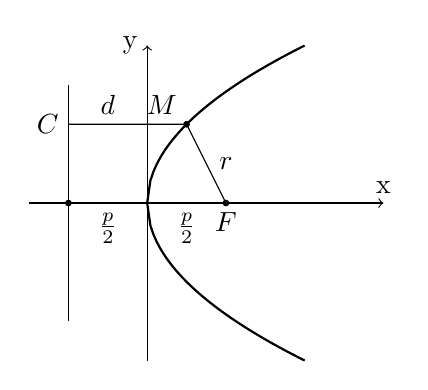
\begin{tikzpicture}[scale=0.5]
		\draw[->] (-3,0) -- (6,0)node[above]{x};
		\draw[->] (0,-4) -- (0,4)node[left]{y};
		
		\draw (-2, 3) -- (-2,-3);	
		\filldraw[black] (-2,0) circle(2pt);
		\filldraw[black] (2,0) circle(2pt);
		\draw (-1,0)node[below]{$\frac{p}{2}$};
		\draw (1,0)node[below]{$\frac{p}{2}$};
		\draw (-2,2)node[left]{$C$} -- (1,2)node[above left]{$M$} -- (2,0)node[below]{$F$};
		\filldraw[black] (1,2) circle(2pt);
		\draw(-1,2)node[above]{$d$};
		\draw(2,1)node{$r$};
			
		\draw[domain=0:4, samples=50, thick] plot ({\x},{sqrt(4*\x)});
		\draw[domain=0:4, samples=50, thick] plot ({\x},{-sqrt(4*\x)});
	\end{tikzpicture}
}\parbox{\textwidth - 5cm}{
	Отримали \textbf{канонічне рівняння
	параболи}: $y =2px$, де $p$ ---
	параметр, $p > 0$.
	Очевидно, що $x \geqslant 0 $. Отже,
	парабола розташована праворуч від
	осі $OY$. З отриманого рівняння
	випливає, що для довільного значення
	$x$ існує два протилежні значення $y$:
	$y = \pm\sqrt{2px}$, а це означає, що
	парабола симетрична відносно осі $OX$ (осі параболи). Парабола проходить через
	точку $O(0,0)$, яка називається її вершиною. Якщо $x \rightarrow +\infty$, то
	$y \rightarrow +\infty$, що означає, що вітки параболи простягаються в нескінченність. 
}

\section{Ексцентриситет і директриси еліпса і гіперболи}

\begin{definition}
	Величина $\varepsilon = \dfrac{c}{a}$ --- це \textbf{ексцентриситет еліпса} і \textbf{ексцентриситет гіперболи}.
\end{definition}

Для еліпса $\varepsilon = \dfrac{c}{a} = \dfrac{\sqrt{a^2 - b^2}}{a} = \sqrt{1-\dfrac{b^2}{a^2}}$,
тому $\varepsilon \in [0;1)$. Якщо $\varepsilon = 0$, то це
означає, що $a=b$ і $c=0$, тобто фокуси еліпса збігаються, і еліпс перетворюється
в коло. Ексцентриситет характеризує форму даної кривої. Чим більше $\varepsilon$, тим
більше еліпс “сплющується” по осі OY.

Для гіперболи $\varepsilon = \dfrac{c}{a} = \dfrac{\sqrt{a^2 + b^2}}{a} = \sqrt{1+\dfrac{b^2}{a^2}}$,
тобто $\varepsilon \in (1;+\infty)$. Із зростанням $\varepsilon$ гілки гіперболи “розпрямлюються”.

\begin{definition}
	\textbf{Директриса еліпса (директриса гіперболи)} --- це дві прямі, які
	перпендикулярні фокальній осі (тобто до осі, на якій розміщені фокуси) і
	знаходяться на відстані $\dfrac{a}{\varepsilon}$ від центра кривої.
\end{definition}

У вибраній системі координат директриси еліпса та гіперболи паралельні осі
$OY$ і не перетинають самі криві. Отже, рівняння директрис $D_1$ і $D_2$ для цих двох
кривих мають вигляд: $x = \pm\dfrac{a}{\varepsilon}$ або $x = \pm\dfrac{a^2}{c}$.

Для еліпса $a > c \Rightarrow \dfrac{a}{c} > 1$, тому $\dfrac{a^2}{c} = \dfrac{aa}{c} > a$
(враховано, що $\varepsilon = \dfrac{c}{a}$ і $0 \leqslant \varepsilon < 1$). Це
означає, що директриси еліпса лежать поза його межами.

Аналогічно для гіперболи $a < c \Rightarrow \dfrac{a}{c} < 1$ і $\dfrac{a^2}{c} = \dfrac{aa}{c} < a$,
тобто директриси гіперболи знаходяться між її гілками.

Для доведення теореми про зв’язок між поняттями ексцентриситет і
директриса розв’яжемо наступну задачу.

\begin{problem}
	Довести, що фокальні радіуси $r_1$ і $r_2$ довільної точки еліпса мають
	вигляд: $r_1 = a + \varepsilon x$, $r_2 = a - \varepsilon x$. 
\end{problem}
\begin{solution}
	Нехай точка $M(x,y)$ --- довільна точка еліпса. Тоді її координати
	задовольняють канонічне рівняння еліпса $\dfrac{x^2}{a^2} + \dfrac{y^2}{b^2} = 1$. Звідси $y^2 = b^2(1-\dfrac{x^2}{a^2})$
	або $y^2 = \dfrac{b^2}{a^2}(a^2-x^2)$. Знайдемо фокальний радіус $r_1$:

	$$r_1 = |F_1M| = \sqrt{(x+c)^2 + y^2} = \sqrt{x^2 + 2xc + c^2 + \dfrac{b^2}{a^2}(a^2-x^2)} =$$

	$$= \sqrt{x^2 + 2xc + c^2 + \dfrac{a^2-c^2}{a^2}(a^2-x^2)} = \sqrt{x^2 + 2xc + c^2 + (1-\dfrac{c^2}{a^2})(a^2-x^2)} =$$

	$$\sqrt{a^2 + 2xc + \dfrac{c^2}{a^2}x^2} = \sqrt{(a + \dfrac{c}{a}x)^2} = |a + \dfrac{c}{a}x| = |a + \varepsilon x|.$$

	Знайдемо знак виразу $a + \varepsilon x$. Оскільки $\dfrac{c}{a} < 1$ і $|x| \leqslant a$, то $|\dfrac{c}{a}x| < a$.
	Тому $a + \dfrac{c}{a}x > 0$, тобто $a + \varepsilon x > 0$ і $r_1 = a + \varepsilon x$, що і треба було довести. Фокальний
	радіус $r_2$ знаходиться аналогічно.
\end{solution}

Зауважимо, що для гіперболи аналогічними міркуваннями можна отримати: $r_1 = \varepsilon x + a$, $r_2 = \varepsilon x - a$.

\begin{theorem}
	Якщо $M(x,y)$ --- довільна точка еліпса чи гіперболи, $r_1$ і $r_2$ --- її
	фокальні радіуси, $\rho(M,D_1)$ і $\rho(M,D_2)$ --- відстані від точки $M$ до відповідної
	директриси, то має місце співвідношення:
	
	$$\dfrac{r_1}{\rho(M,D_1)} = \dfrac{r_2}{\rho(M,D_2)} = \varepsilon$$
\end{theorem}
\begin{proof}(проведемо для еліпса):
	
	$$\dfrac{r_1}{\rho(M,D_1)} = \dfrac{r_1}{d_1} = \dfrac{a + \varepsilon x}{x + \dfrac{a}{\varepsilon}}
	= \varepsilon\dfrac{a + \varepsilon x}{\varepsilon x + a} = \varepsilon,$$
	
	$$\dfrac{r_2}{\rho(M,D_2)} = \dfrac{r_2}{d_2} = \dfrac{a - \varepsilon x}{x - \dfrac{a}{\varepsilon}}
	= \varepsilon\dfrac{a - \varepsilon x}{\varepsilon x - a} = \varepsilon,$$

	\begin{center}
		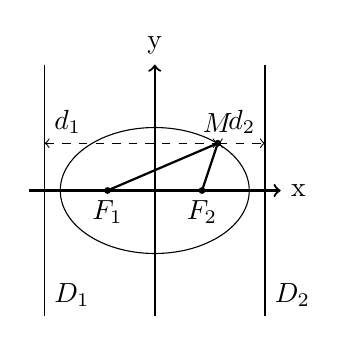
\begin{tikzpicture}[scale=0.4]
			\draw[->, thick] (-4,0) -- (4,0)node[right]{x};
			\draw[->, thick] (0,-4) -- (0,4)node[above]{y};
		
			\draw (0,0) ellipse (3cm and 2cm);
			
			\draw (-3.5,4) -- (-3.5,-4)node[above right]{$D_1$};
			\draw (3.5,4) -- (3.5,-4)node[above right]{$D_2$};
			\draw[thick] (-1.5,0)circle(2pt)node[below]{$F_1$} -- (2,1.5)circle(2pt)node[above]{$M$} -- (1.5,0)circle(2pt)node[below]{$F_2$};
			\draw[dashed, <->] (-3.5,1.5)node[above right]{$d_1$} -- (2,1.5);
			\draw[dashed, <->] (2,1.5) -- (3.5,1.5)node[above left]{$d_2$};
		\end{tikzpicture}
		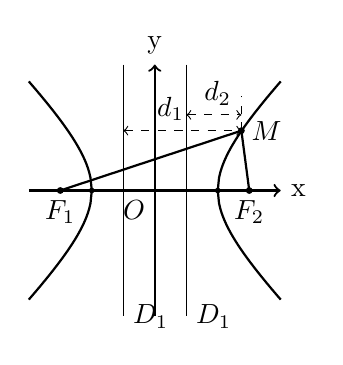
\begin{tikzpicture}[scale=0.4]
			\draw[->, thick] (-4,0) -- (4,0)node[right]{x};
			\draw[->, thick] (0,-4) -- (0,4)node[above]{y};
			%\draw[gray, dashed] (-4,-4) grid (4,4);
		
			\def\a{2};
			\def\b{2};
		
			\draw[domain=\a:4, samples=50, thick] plot (\x,{(\b/\a)*sqrt(\x^2 - \a^2)});
			\draw[domain=\a:4, samples=50, thick] plot (\x,{-(\b/\a)*sqrt(\x^2 - \a^2)});
			\draw[domain=\a:4, samples=50, thick] plot ({-\x},{(\b/\a)*sqrt(\x^2 - \a^2)});
			\draw[domain=\a:4, samples=50, thick] plot ({-\x},{-(\b/\a)*sqrt(\x^2 - \a^2)});
			
			\filldraw[black] (2,0) circle(2pt);
			\filldraw[black] (-2,0) circle(2pt);
			
			\draw (-1,4) -- (-1,-4)node[right]{$D_1$};
			\draw (1,4) -- (1,-4)node[right]{$D_1$};
			%\draw (-3,0)node[below]{$F_1$} -- (2.75,2)node[right]{$M$} -- (3,0)node[below]{$F_2$};
			\filldraw[black, thick] (-3,0)circle(2pt)node[below]{$F_1$} -- (2.75,1.9)circle(2pt)node[right]{$M$} -- (3,0)circle(2pt)node[below]{$F_2$};

			\draw (0,0)node[below left]{$O$};
			
			\draw[dashed] (2.75,1.9) -- (2.75,3);
			
			\draw[dashed, <->] (-1,1.9) -- (0.5,1.9)node[above]{$d_1$} -- (2.75,1.9);
			\draw[dashed, <->] (1,2.4) -- (2,2.4)node[above]{$d_2$} -- (2.75,2.4);
		\end{tikzpicture}
	\end{center}
	
\end{proof}

\begin{remark}
	 Для довільної точки параболи $\dfrac{r}{d} = 1$, тобто $\epsilon = 1$. 
\end{remark}

\section{Рівняння дотичної до кривої другого порядку}

Побудуємо рівняння дотичної до еліпса $\dfrac{x^2}{a^2} + \dfrac{y^2}{b^2} = 1$ в точці $M_0(x_0,y_0)$.
Нехай $y_0 \neq 0$, тобто точка $M_0$ не співпадає ні з однією з вершин еліпса $A_1(-a,0)$
та $A_2(a,0)$. У цьому випадку рівняння $\dfrac{x^2}{a^2} + \dfrac{y^2}{b^2} = 1$ неявно задає функцію $y = y(x)$,
$-a < x < a$, графік якої проходить через точку $M_0(x_0,y_0)$ і співпадає з верхньою
(при $y_0 > 0$) чи нижньою (при $y_0 < 0$) половиною еліпса.

Скористаємось відомим із шкільного курсу рівнянням дотичної до графіка
функції $y = f(x)$ в точці з абсцисою $x_0$, яке має вигляд: $y = y_0 + f'(x_0)(x - x_0)$.

Якщо продиференціювати за $x$ тотожність $\dfrac{x^2}{a^2} + \dfrac{y^2(x)}{b^2} = 1$, то отримаємо
рівняння 

$$\dfrac{2x}{a^2} + \dfrac{2yy'(x)}{b^2} = 0,$$ 

\begin{center}
або
\end{center}

$$b^2x + a^2yy'(x) = 0,$$

\begin{center}
тобто 
\end{center}

$$y'(x) = -\dfrac{b^2x}{a^2y}.$$

Якщо підставити значення $y'(x_0) = -\dfrac{b^2x_0}{a^2y_0}$
у рівняння дотичної, то отримаємо рівняння:

$$y = y_0 -\dfrac{b^2x_0}{a^2y_0}(x - x_0).$$

Виконаємо нескладні перетворення:

$$y = y_0 -\dfrac{b^2x_0x}{a^2y_0} +\dfrac{b^2x_0^2}{a^2y_0}, a^2y_0y = a^2y_0^2 - b^2x_0x + b^2x_0^2.$$

Якщо поділити обидві частини рівняння на $a^2b^2$ та врахувати те, що
$\dfrac{x_0^2}{a^2} + \dfrac{y_0^2}{b^2} = 1$ (точка $M_0(x_0,y_0)$ лежить на еліпсі), то отримаємо:

$$\dfrac{y_0y}{b^2} = \dfrac{y_0^2}{b^2} - \dfrac{x_0x}{a^2} + \dfrac{x_0^2}{a^2}.$$

Звідси рівняння дотичної до еліпса в точці $M_0(x_0,y_0)$ має вигляд:

$$\dfrac{x_0x}{a^2} + \dfrac{y_0y}{b^2} = 1.$$

Аналогічно можна вивести рівняння дотичної, проведеної до гіперболи та
параболи в точці $M_0(x_0,y_0)$, відповідно: 

$$\dfrac{x_0x}{a^2} - \dfrac{y_0y}{b^2} = 1,$$

$$yy_0 = p(x + x_0).$$




